\documentclass[border=10pt]{standalone}
\usepackage[utf8]{inputenc}
\usepackage[T1]{fontenc}
\usepackage{libertine}
\usepackage{tikz}
\usetikzlibrary{positioning,arrows.meta,shapes.geometric,fit,backgrounds,calc}

\begin{document}
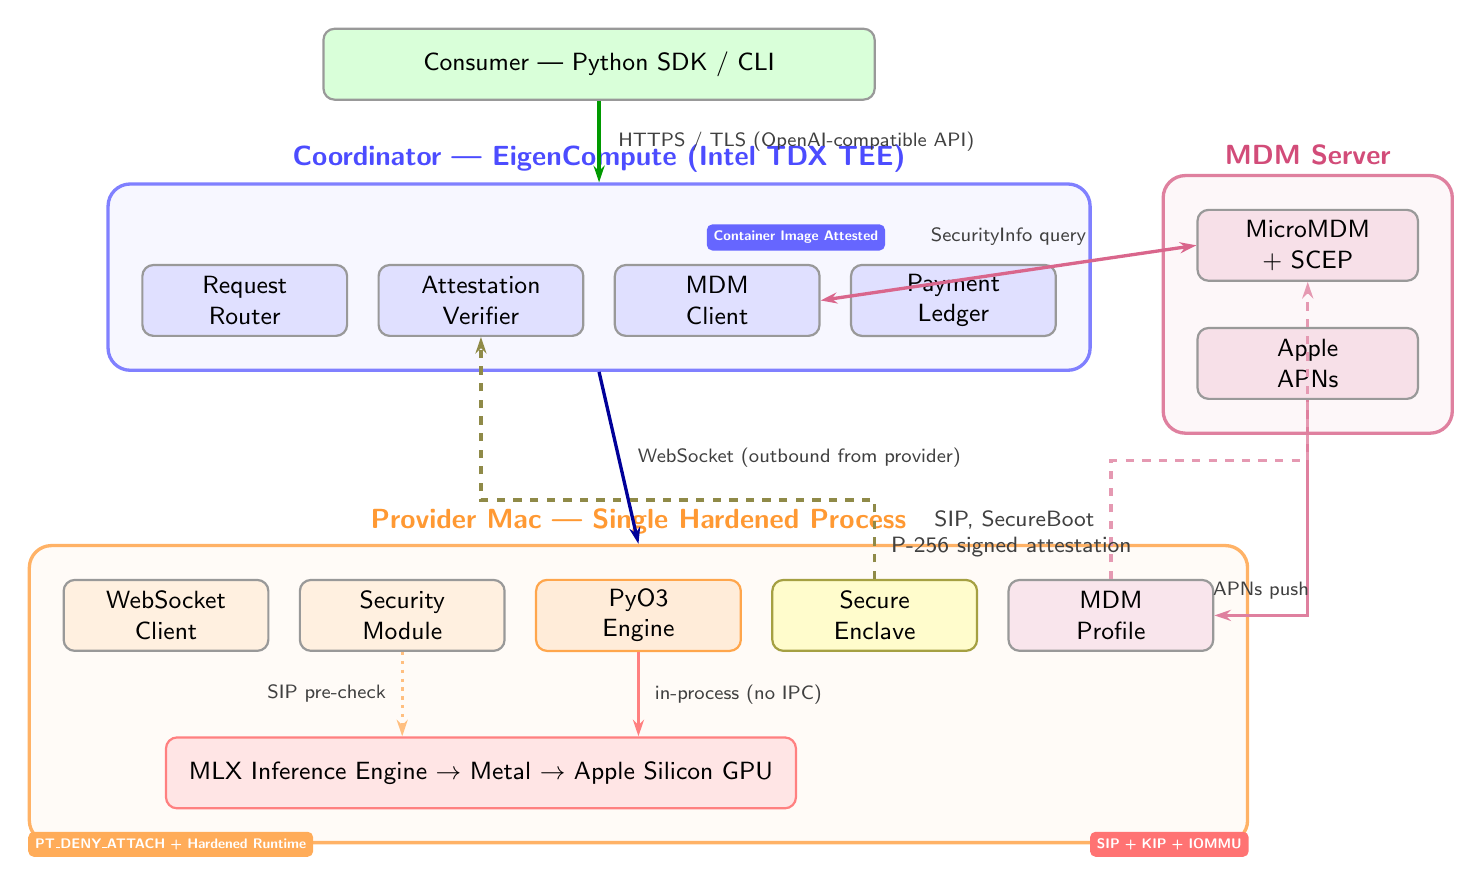
\begin{tikzpicture}[
    % Styles
    component/.style={
        draw=gray!80, thick, rounded corners=4pt,
        fill=#1, minimum width=2.6cm, minimum height=0.9cm,
        font=\small\sffamily, align=center,
    },
    component/.default={white},
    groupbox/.style={
        draw=#1, very thick, rounded corners=8pt,
        inner sep=12pt,
    },
    groupbox/.default={gray!50},
    arr/.style={-{Stealth[length=6pt,width=4pt]}, very thick, #1},
    arr/.default={gray!60},
    biarr/.style={{Stealth[length=6pt,width=4pt]}-{Stealth[length=6pt,width=4pt]}, very thick, #1},
    biarr/.default={gray!60},
    lbl/.style={font=\scriptsize\sffamily, #1},
    lbl/.default={gray!50!black},
    grouptitle/.style={font=\normalsize\sffamily\bfseries, #1},
    grouptitle/.default={black},
    badge/.style={
        font=\tiny\sffamily\bfseries, rounded corners=2pt,
        fill=#1, text=white, inner sep=2.5pt,
    },
]

% ================================================================
% ROW 1: CONSUMER
% ================================================================
\node[component=green!15, minimum width=7cm] (consumer) at (0, 0)
    {Consumer --- Python SDK / CLI};

% ================================================================
% ROW 2: COORDINATOR (EigenCompute TEE)
% ================================================================
\node[component=blue!12] (router) at (-4.5, -3) {Request\\Router};
\node[component=blue!12] (attverify) at (-1.5, -3) {Attestation\\Verifier};
\node[component=blue!12] (mdmclient) at (1.5, -3) {MDM\\Client};
\node[component=blue!12] (payments) at (4.5, -3) {Payment\\Ledger};

% Invisible spacer above components for badge room
\node[minimum height=0.5cm, minimum width=1cm] (coordspacer) at (4.5, -2.2) {};
\begin{scope}[on background layer]
    \node[groupbox=blue!50, fill=blue!3,
          fit=(router)(attverify)(mdmclient)(payments)(coordspacer),
          label={[grouptitle=blue!70]above:{Coordinator --- EigenCompute (Intel TDX TEE)}}
         ] (coordbox) {};
\end{scope}
\node[badge=blue!60] at (2.5, -2.2) {Container Image Attested};

% ================================================================
% ROW 3: PROVIDER MAC
% ================================================================
\node[component=orange!12] (wsclient) at (-5.5, -7) {WebSocket\\Client};
\node[component=orange!12] (secmod) at (-2.5, -7) {Security\\Module};
\node[component=orange!15, draw=orange!70] (pyo3) at (0.5, -7) {PyO3\\Engine};
\node[component=yellow!20, draw=yellow!60!black] (enclave) at (3.5, -7) {Secure\\Enclave};

\node[component=red!10, draw=red!50, minimum width=8cm, minimum height=0.9cm]
    (mlx) at (-1.5, -9) {MLX Inference Engine $\to$ Metal $\to$ Apple Silicon GPU};

\node[component=purple!10] (mdmprofile) at (6.5, -7) {MDM\\Profile};

\begin{scope}[on background layer]
    \node[groupbox=orange!60, fill=orange!3,
          fit=(wsclient)(secmod)(pyo3)(enclave)(mlx)(mdmprofile),
          label={[grouptitle=orange!80]above:{Provider Mac --- Single Hardened Process}}
         ] (provbox) {};
\end{scope}

\node[badge=orange!65, anchor=west] at (provbox.south west) {PT\_DENY\_ATTACH + Hardened Runtime};
\node[badge=red!55, anchor=east] at (provbox.south east) {SIP + KIP + IOMMU};

% ================================================================
% SIDE: MDM SERVER
% ================================================================
\node[component=purple!12, minimum width=2.8cm] (mdmserver) at (9, -2.3) {MicroMDM\\+ SCEP};
\node[component=purple!12, minimum width=2.8cm] (apns) at (9, -3.8) {Apple\\APNs};

\begin{scope}[on background layer]
    \node[groupbox=purple!50, fill=purple!3,
          fit=(mdmserver)(apns),
          label={[grouptitle=purple!70]above:{MDM Server}}
         ] (mdmbox) {};
\end{scope}

% ================================================================
% ARROWS
% ================================================================

% Consumer -> Coordinator
\draw[arr=green!60!black]
    (consumer.south) -- (coordbox.north)
    node[lbl, midway, right=3pt] {HTTPS / TLS (OpenAI-compatible API)};

% Coordinator -> Provider
\draw[arr=blue!60!black]
    (coordbox.south) -- (provbox.north)
    node[lbl, midway, right=3pt] {WebSocket (outbound from provider)};

% MDM Client <-> MDM Server
\draw[biarr=purple!60]
    (mdmclient.east) -- (mdmserver.west)
    node[lbl, midway, above=6pt] {SecurityInfo query};

% APNs -> MDM Profile (push notification)
\draw[arr=purple!50]
    (apns.south) |- (mdmprofile.east)
    node[lbl, pos=0.75, above=2pt] {APNs push};

% MDM Profile -> MDM Server (response path)
\draw[arr=purple!40, dashed]
    (mdmprofile.north) -- ++(0, 1.5)
    node[lbl, left=2pt, pos=0.5] {\footnotesize SIP, SecureBoot}
    -| (mdmserver.south);

% Secure Enclave -> Attestation Verifier
\draw[arr=yellow!50!black, dashed]
    (enclave.north) -- ++(0, 1.0)
    node[lbl, right=2pt, pos=0.4] {\footnotesize P-256 signed attestation}
    -| (attverify.south);

% PyO3 -> MLX (in-process call)
\draw[arr=red!50]
    (pyo3.south) -- (mlx.north-|pyo3.south)
    node[lbl, midway, right=2pt] {in-process (no IPC)};

% Security Module -> MLX (SIP pre-check)
\draw[arr=orange!50, dotted]
    (secmod.south) -- (mlx.north-|secmod.south)
    node[lbl, midway, left=2pt] {SIP pre-check};

\end{tikzpicture}
\end{document}
